\problemname{\problemyamlname}


\begin{wrapfigure}{r}{5.5cm}
    \centering
    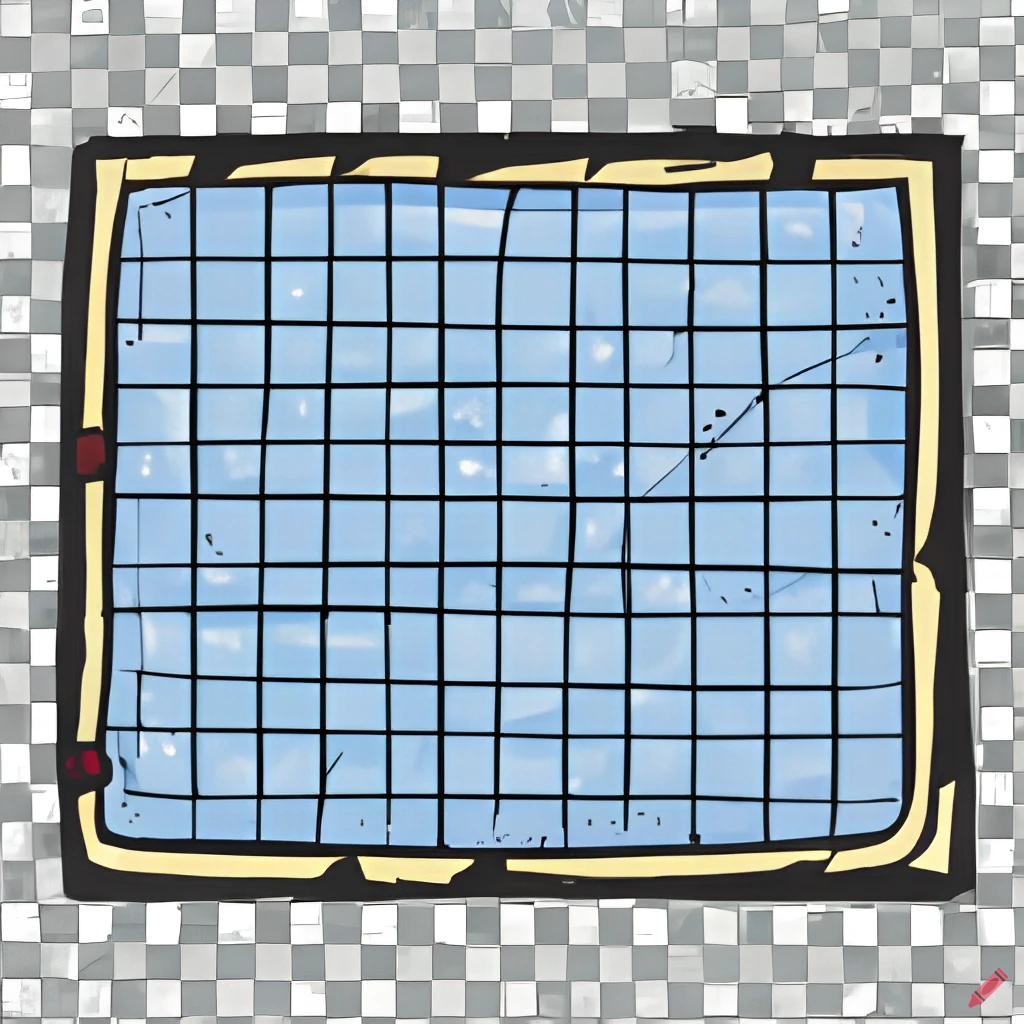
\includegraphics[width=5.5cm]{ravitaillement.jpg}
\end{wrapfigure}

You have been freshly employed at an important development and optimization job at the Center for Activities and Recreation during Weekends of the Adventurous (CARWA).
The weekend is approaching quickly, and one of the activities is happening at Delft.
The teams and coaches have already gone towards their destination, but we have a problem.
No one has thought about the refreshments!
Delft is a true maze, a big rectangle composed of squared zones, and it would be dangerous to leave our teams without such a support.

We need your help to find the ideal size of a refreshments camp in the city without bothering the activity of the teams.

You have at your disposition the name of each team, their position in the city, and if it's a team of candidates or coaches.
The city is composed of $m \times m$ small square zones on your map.
A team of candidates can't find itself on only one square, but a single team of coaches can be dispersed over multiple squares.
Two teams can never be found on the same square, but a square can be empty.

Your goal is to find the largest rectangle in Delft where only teams of coaches can be found, so that they can create the largest refreshment camps.
It imperatively needs to be a rectangle, because of the complexity of navigating Delft.
Once you've found this rectangle, indicate to your superiors how many teams will be mobilized to establish this refreshment.

\begin{Input}
	The input consists of :
	\begin{itemize}
		\item One line with three integers $n$, $m$ and $k$ ($1 \le n,m \le 10^3$, $1 \le k \le 20$), respectively the number of zones in a line, the number of zones in a column, and the number of teams of coaches present on the ground.
		\item $n$ lines, where each line contains $m$ names separated by a space, of the form ``\verb|name_1 name_2 ... name_m|''. The $j$\textsuperscript{th} name of the $i$\textsuperscript{th} line represents the team in the zone $(i,j)$,
		\item $k$ lines, where a line is the name of a team of coaches.
	\end{itemize}
	The names are composed of letters of the alphabet, in lowercase, and without accents or special characters.
	When a square isn't occupied by any teams, the corresponding name will be ``\verb|null|''.
\end{Input}

\begin{Output}
	 The number of zones in the largest rectangle composed only of zones occupied by coaches.
\end{Output}
